\hypertarget{on-na-jamais-uxe9tuxe9-autant-uxe0-la-plage-en-hiver}{%
\section{On n'a jamais été autant à la plage en
hiver}\label{on-na-jamais-uxe9tuxe9-autant-uxe0-la-plage-en-hiver}}

\emph{Jeudi 26 juillet 2018}

Sur les conseils avisés de nos hôtes, Svenja et Rémi, nous avons exploré
différents points touristiques de la région de Sydney. Si on voulait
résumer notre programme en un seul mot, ce serait \textbf{plage}. Malgré
l'hiver, nos déplacements nous ont tous amené au point de rencontre
entre le sable, les vagues et le ciel dont la Nouvelle-Galles du Sud
regorge.

L'une des premières étapes sur notre chemin a été la découverte du
quartier de Darlinghurst, où nous logeons. Comme Elida l'évoquait à
travers le titre de l'\href{/arrivee-australie.html}{article précédent},
on croise toutes sortes d'oiseaux à Sydney, bien plus que ce dont nous
avons l'habitude. Que ce soient les cacatoès, les kookaburras ou les
"petits gris", les derniers descendants des dinosaures nous ont séduits
ici ! Quoi de plus agréable que de prendre le petit déjeuner avec des
perroquets ?

\begin{figure}
\centering
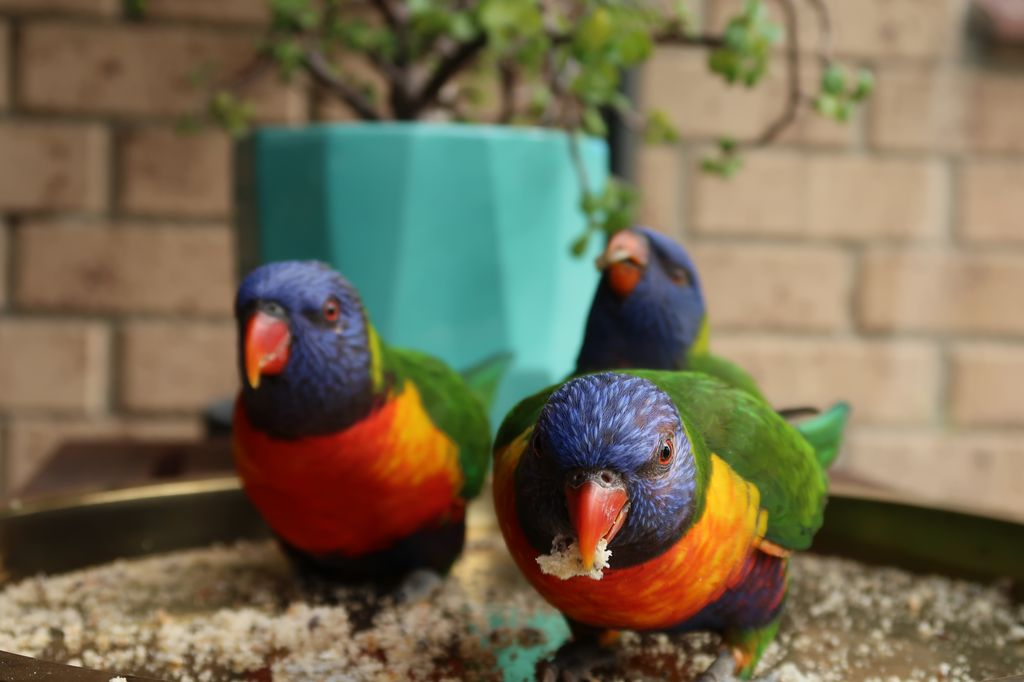
\includegraphics{images/20180726_perroquets.JPG}
\caption{Le gang des trois perroquets, prêts à tout pour obtenir de la
mie de pain au petit déjeuner.}
\end{figure}

Pour en revenir au sujet, nous avons donc découvert les endroits
suivants :

\begin{itemize}
\tightlist
\item
  Bondi beach : la plage "légendaire" de l'été australien, mais qui
  offre également une belle promenade en bordure de mer pour admirer le
  relief ; on a même eu la chance d'y apercevoir des baleines !
\item
  Watson's bay : l'un des caps qui délimite la baie de Sydney par le
  sud, là aussi l'occasion de marcher le long de jolis sentiers
\item
  Manly : nommée par le capitaine Arthur Philipp en raison de la
  virilité des locaux, c'est l'anti-Watson's bay, duquel nous avons
  marché de crique en crique et à travers le Sydney Harbour National
  Park, jusqu'à atteindre Spit Bridge (une balade mémorable qu'on a
  terminé à la lampe torche...)
\item
  Balmoral : abritée dans la baie de Sydney, cette partie de la côte
  offre des vues magnifiques sur le centre-ville et son port
\end{itemize}

Ces promenades nous ont permis de mieux comprendre ce qui fait la
spécificité et l'art de vivre de Sydney : ville cosmopolite, moderne et
riche d'histoire, mais surtout très près de sa nature et de sa faune
abondante. De nombreuses mesures semblent d'ailleurs constamment mises
en œuvre pour protéger la nature : panneaux signalant les interdits mais
aussi les types de plantes, poubelles avec tri et recyclage, zones de
régénération du "bush" où l'on se nettoie les chaussures pour éviter de
transporter des spores exogènes, zones de végétation replantée, plages
où les chiens ne sont pas autorisés... Et cela a l'air de marcher : on
trouve très peu de déchets abandonnées, les côtes sont très propres avec
une faune et une flore très riches et variées et donc un véritable
bonheur à explorer.

\begin{figure}
\centering
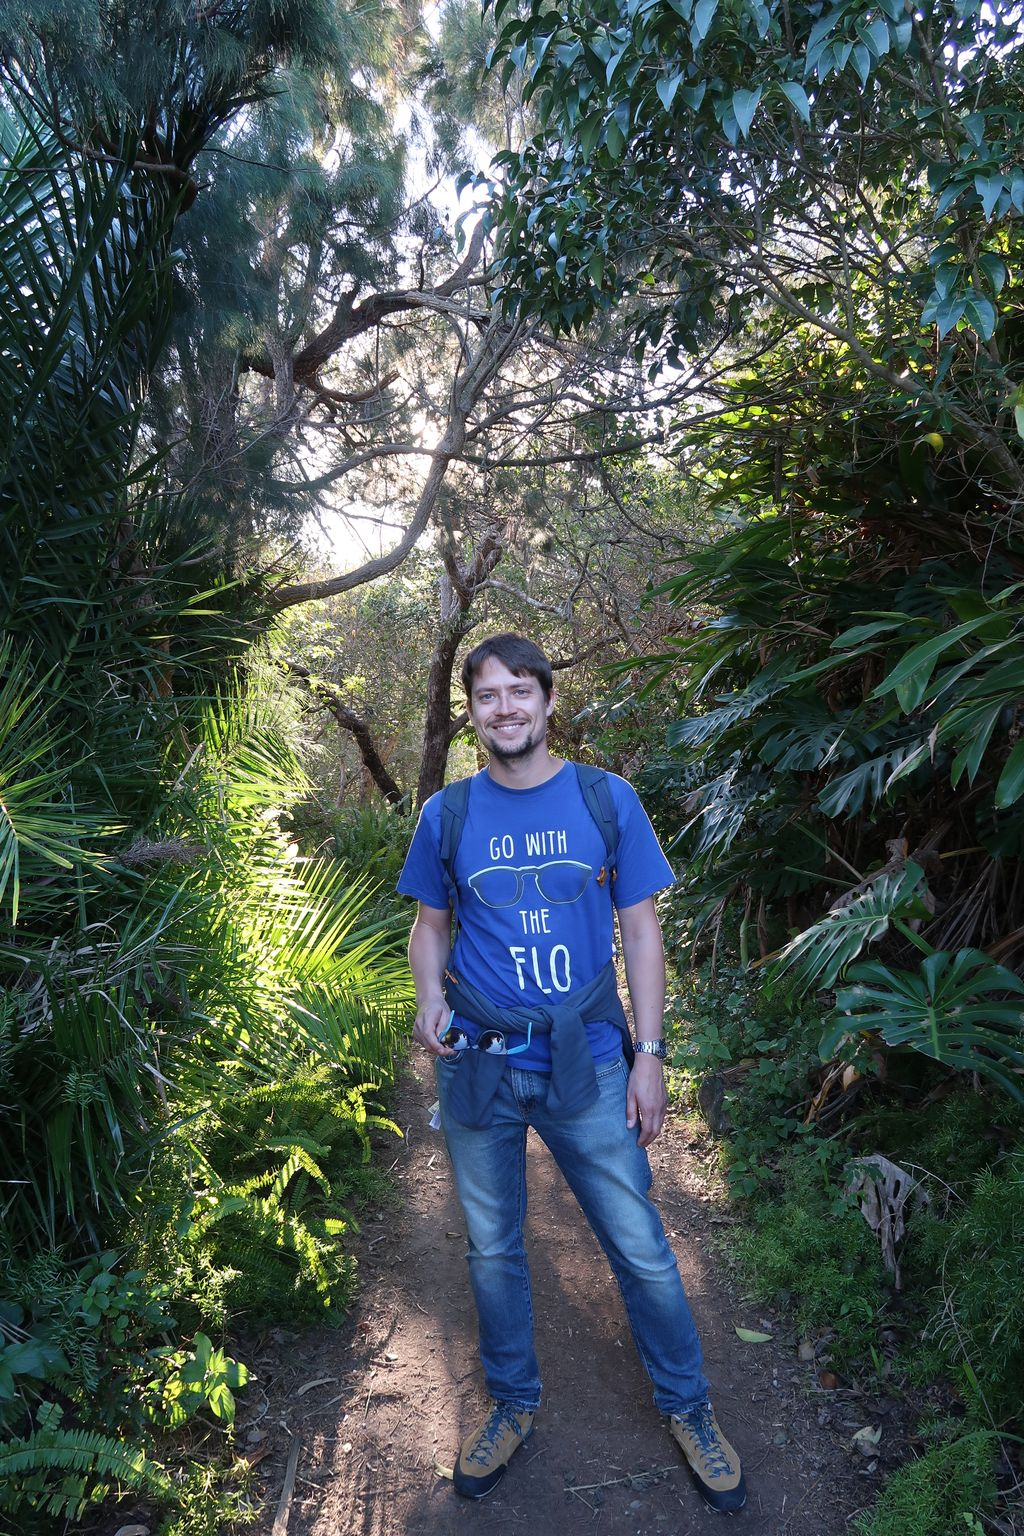
\includegraphics{images/20180726_bush.JPG}
\caption{Le bush australien par l'exemple.}
\end{figure}

Le temps d'un week-end, Svenja et Rémi nous ont emmenés un peu plus au
nord de Sydney, sur la Central Coast. La route donne le ton : très
rapidement à la sortie de la ville on se retrouve sur des voies
découpées au milieu de la montagne, puis nous commençons à apercevoir à
chaque virage le scintillement des vagues, et des plages plus belles les
unes que les autres. On s'arrêtera à des plages aux noms évocateurs :
Pearl Beach, Copacabana,... Les balades sur le sable sont très agréables
même si parfois un peu fraîches (n'oublions pas qu'on est en plein hiver
ici), et la lumière du coucher de soleil sur la côte découpée du Bouddi
National Park nous émerveille.

Voilà pour ce premier aperçu de notre voyage en Australie, on continue
bientôt pour un road-trip sur la Great Ocean Road !

\emph{Florian et Elida}
